\section*{Úvod}
Pravdou je, že v moderním světě je mnoho problémů, které můžeme vnímat jako bezpečností hrozbu. Jednou z nejskloňovanějších hrozeb v očích odborníků jsou v moderní \textit{post-truth} době dezinformace, ty jsou v rámci momentálně stále probíhající světové pandemie silnou zbraní, prostřednictvím které je možné ovlivnit veřejné mínění, názory a v konečném důsledku tedy i samotné chování jednotlivých lidí. Mnoho subjektů, ať už se jedná o individua, větší skupiny, či dokonce národní/nadnárodní skupiny, které mohou být nezřídkakdy podporovány i státy, se prostřednictvím dezinformací snaží dosáhnout svých cílů nejen na scéně domácí, ale i v zahraničí. Považuji proto za velice důležité o dezinformacích mluvit a zasadit se za osvětovou kampaň, aby proti snaze o použití dezinformací lidé byli více imunní. I z toho důvodu jsem se rozhodl pojednat ve své seminární práci o tématu dezinformací, a to specificky ve světle momentální pandemické situace, práce je tedy zaměřena především na dezinformace spojené s pandemií koronaviru a snahou o jeho zvládnutí (Zde se dá hovořit například o dezinformace směřované vůči vakcínám.).

\section{Pojem dezinformace}

V moderní době internetové, kdy má přibližně 51\% obyvatel přístup k internetu\cite{noauthor_individuals_nodate}, se mohou dezinformace šířit stejnou rychlostí jako opravdivé informace a mnoho lidí tedy může snadlo podlehnout pocitu, že čtou pravdivé informace i když ve skutečnosti se jedná o dezinformace. Jde rovněž důvodně předpokládat, že v současné době, kdy mnoho lidí dma tráví více času než obvykle, bude dopad dezinformací značně vyšší.\\

Než ale přejdu k problematice dezinformací, je potřeba tento pojem nejdříve definovat. Pokud je třeba definovat jakýkoliv pojem, obracím se často na \textit{Oxford dictionary}, učinil jsem tak proto i teď, Oxfordský slovník tedy dezinformace definuje jako: \textit{"false information that is given deliberately"}\cite{noauthor_disinformation_nodate}, v překladu tedy jako \textit{"nepravdivá informace, která je sdělena záměrně}.\\

V této souvislosti je nutné zmínit dvě "podkategorie" dezinformací, a to výše definovanou dezinformaci jakožto úmyslně nepravdivou informaci a dále "misinformaci", či špatnou informaci, která je neúmyslně šířena i když je nepravdivá (chybí tedy aspekt úmyslu sdílet špatnou informaci), nicméně to nic nemění na faktu, že je stále sdílena nepravdivá informace, což v konečném důsledku může vést k úplně stejným výsledkům.\\

Nakonec je potřeba řící, že dezinformace nejsou ničím novým, existují již po celá milénia, nicméně v období před masovým využíváním internetu měly pouze omezený dosah. Postupné zvyšování dostupnosti moderní výpočetní techniky společně s internetem jako takovým umožnilo exponenciální nárůst v olbasti efektivnosti a množství šířených dezimformací. Dá se předpokládat, že k nárůstu šíření dezinformací přispělo především velké množství sociálních sítí, které umožnilo propojení lidí s podobnými zájmy napříč celým světem. Tento fakt ve svém důsledku umožnil subjektům, které chtějí dezinformace šířit, spojení s jinými subjekty s podobnými hodnotami, což v konečném důsledku dále zrychluje šíření dezinformací a zároveň v ně podporuje u těchto subjektů víru, neboť "nejsou sami, kdo si to myslí". Sociální sítě tak mají velkou možnost ovlivňovat celospolečenskou situaci jak v pozitivním, tak i v negativním světle, neboť jejichž prostřednictvím je možné přispívat k diskuzi o směřování společnosti a rovněž i k vnímání jednotlivých témat ze strany společnosti.

\subsection{Dezinformace v době Covidové}

Jednou z největších výzev v době probíhající pandemie COVID-19 byl, je a bude nejen boj proti koronaviru jako takovému, ale i proti dezinformacím, které jsou využíváný pro šíření nepravd či polopravd. Ve veřejném prostoru je možné sledovat mnoho diskuzí nad tím, jak se s dezinformacemi vypořádat.\\

Zdroje informací, a to jak v online prostoru, tak i v rámci televizního a rádiového vysílání, či dokonce v tisku jsou protkané nespočetným množstvím falešných a zavádějících tvrzeních týkajíce se zdroje, způsobu přenášení, závažnosti a v konečném důsledku i léčby virusu a snahy o jeho vymícení. Může se jednat o poměrně neškodná marketingová tvrzení ohledně zdánlivě účinných produktů jako například produkt od UVLEN \textregistered Technologies Korea\cite{uvlen__uvlen_nodate}, u kterého výrobce tvrdí, že má vlastnosti, které odporují základním zákonům fyziky (vlnovou délku světla není možné změnit za pomocí jednoduchého filtru), až po vážné útoky na vědce, a orgány veřejné moci, které mohou vyůstit až v občanskou neposlušnost, jako příklad je možné připomenout nedávný útok na Kapitol zfanatizovaných davem, který se nechal přesvědčit dezinformacemi vyslovenými americkým prezidentem Donaldem Trumpem.\\

V této souvislosti je problémem právě to, že některé z těchto misinformací a dezinformací jsou širší veřejností opravdu považovány za pravdivé a to ať už jsou šířeny úmyslně (v případě dezinformací), či neúmyslně (v případě misinformací). Problémem u obou druhů dezinformací zůstává, že jsou stejně tak dobře schopny klamat a způsobovat újmu. Dezinformace představují pro společnost vážný problém, neboť podkopávají důvěru veřejnosti a zároveň díky svému nadměrnému množství znesnadňují schopnost dohledávat si pravdivé informace a důvěryhodné zdroje. Toto je obzvláštně nebezpečné v období pandemické krize, neboť mnoho dezinformací cílí na podkopání důvěry v protiepidemické opatření, zdravotní systém a očkování (u očkování je nechuť s ním spojená velice výrazná, přičemž argumenty "odmítačů" stojí převážně na nepravdivých informacích).\\ % Udělat vícuc jak lidi mluví o odmítání očkování na Twitteru

WHO problém s dezinformacemi zaměřující se na pandemii koronaviru označuje jako \textit{infodemii} a klade velký důraz na boj proti ní\cite{noauthor_covid-19_nodate}. V této souvislosti pak stanovuje dva velice důležité body v rámci boje proti dezinformacím:

\begin{enumerate}
\item nutnost zjistit, jak se dezinformace šíří,
\item způsob, jakým by na dezinformace měli světové vlády a korporace reagovat.	
\end{enumerate}

%\newpage

Způsob, jak proti dezinformacím bojovat práce načrtává v kapitole 3, nicméně již v této části práce je nutné řící, že reakce, jakožto bod druhý v řetězci řešení problému s dezinformacemi vyžaduje znalosti o bodu prvním, aby bylo možné navrhnout funkční způsoby určené právě k tomu, jak se dezinformacemi bojovat.

%\subsection{Studie, sdílení dezinformací prostřednictvím Twitteru}
%\subsection{Google Trends a dezinformace}

\section{Zdroje dezinformací, aneb jak se dezinformace šíří}

Misinformace a dezinformace bují nejvíce v dobách krizí a nejistot, dezinformace týkající se zdraví tedy bují nejvíce v dobách krize, která se zdraví obyvatel přímo týká, neboť se jedná o situace, ve kterých jsou obyvatelé znepokojení a bojí se dopadu na svoje vlastní zdraví a blahobyt. Není asi nasnadě říci, že právě v takové situaci se momentálně nacházíme. Právě v takovýchto situacích je žízeň po zázračném léku, který nemoc přes noc vymítí, či po ujištění, že vlastně žádná krizová situace neexistuje největší a dezinformace tak mají nejvíce prostoru k pronikání do našich newsfeedů a k našemu následnému ovlivňování.\\

O závažnosti tohoto tématu svědčí i fakt, že na toto téma je v poslední době vypracováno mnoho studií, které se zabívají právě body stanovenými v kapitole 1, tedy zdrojem dezinformací a potenciálními přístupy k této problematice, respektive k jejímu řešení. Zajímavou studií týkající se problematiky je \textit{Types, sources, and claims of COVID-19 misinformation} od Dr. J. Scott Brennen a kol. z Reuters Institute for the Study of Journalism and the Oxford Internet Institute\cite{noauthor_types_nodate}, která poskytuje pohled na nynější alarmující informační stav ve společnosti. Pro toto zjištění však není nutné studovat vydané studie, je možné použít veřejně dostupných prostředků, pomocí kterých si každý člověk může zjistit rozsah dezinformací v naší společnosti. Kratší analýzu nad tímto problémem za použití několika předem vydefinovaných klíčových slov poskytuji níže.\\

\subsection{Studie, sdílení dezinformací prostřednictvím Twitteru}

Jako první způsob ověření hypotézy, že dezinformace jsou v dnešním veřejném informačním prostoru všudypřítomné může sloužit prosté vyhledávání \# hashtagů na Twitteru.\\

\textbf{Předem vydefinovaná klíčová slova:} \textit{\textbf{\#}fakevirus}, \textit{\textbf{\#}fakecovid}, \textit{\textbf{\#}nomasks}, \textit{\textbf{\#}novaccine}, \textit{\textbf{\#}endthelockdown}, \textit{\textbf{\#}scamdemic}, \textit{\textbf{\#}covidhoax} a mnoho dalších.\\

Příklady fakenews tweetu:\\

Samozřejmě pro odpovídající výsledek, by musel být dataset mnohem větší, toto bylo pouze pro ilustraci.\\

Jako doklad mého tvrzení pak může sloužit například výzkum: https://arxiv.org/pdf/2005.05710.pdf, který dělal analýzu i na základě klasických klíčových slov, jako: \textit{\textbf{\#}covid19}, či \textit{\textbf{\#}coronavirus}.\\

\textbf{Výsledek:}
\subsection{Google Trends a dezinformace}

Rovněž si hypotézu/rovněž je si možné potvrdit hypotézu prostřednictvím stránky Google Trends, do které zadáme stejná klíčová slova a můžeme se podívat na frekvenci jejich vyhledávání.\\

\textbf{Výsledek:}

Například. Obrázek č.~\ref{fig:tux}

\begin{figure}[htbp]
  \centering
  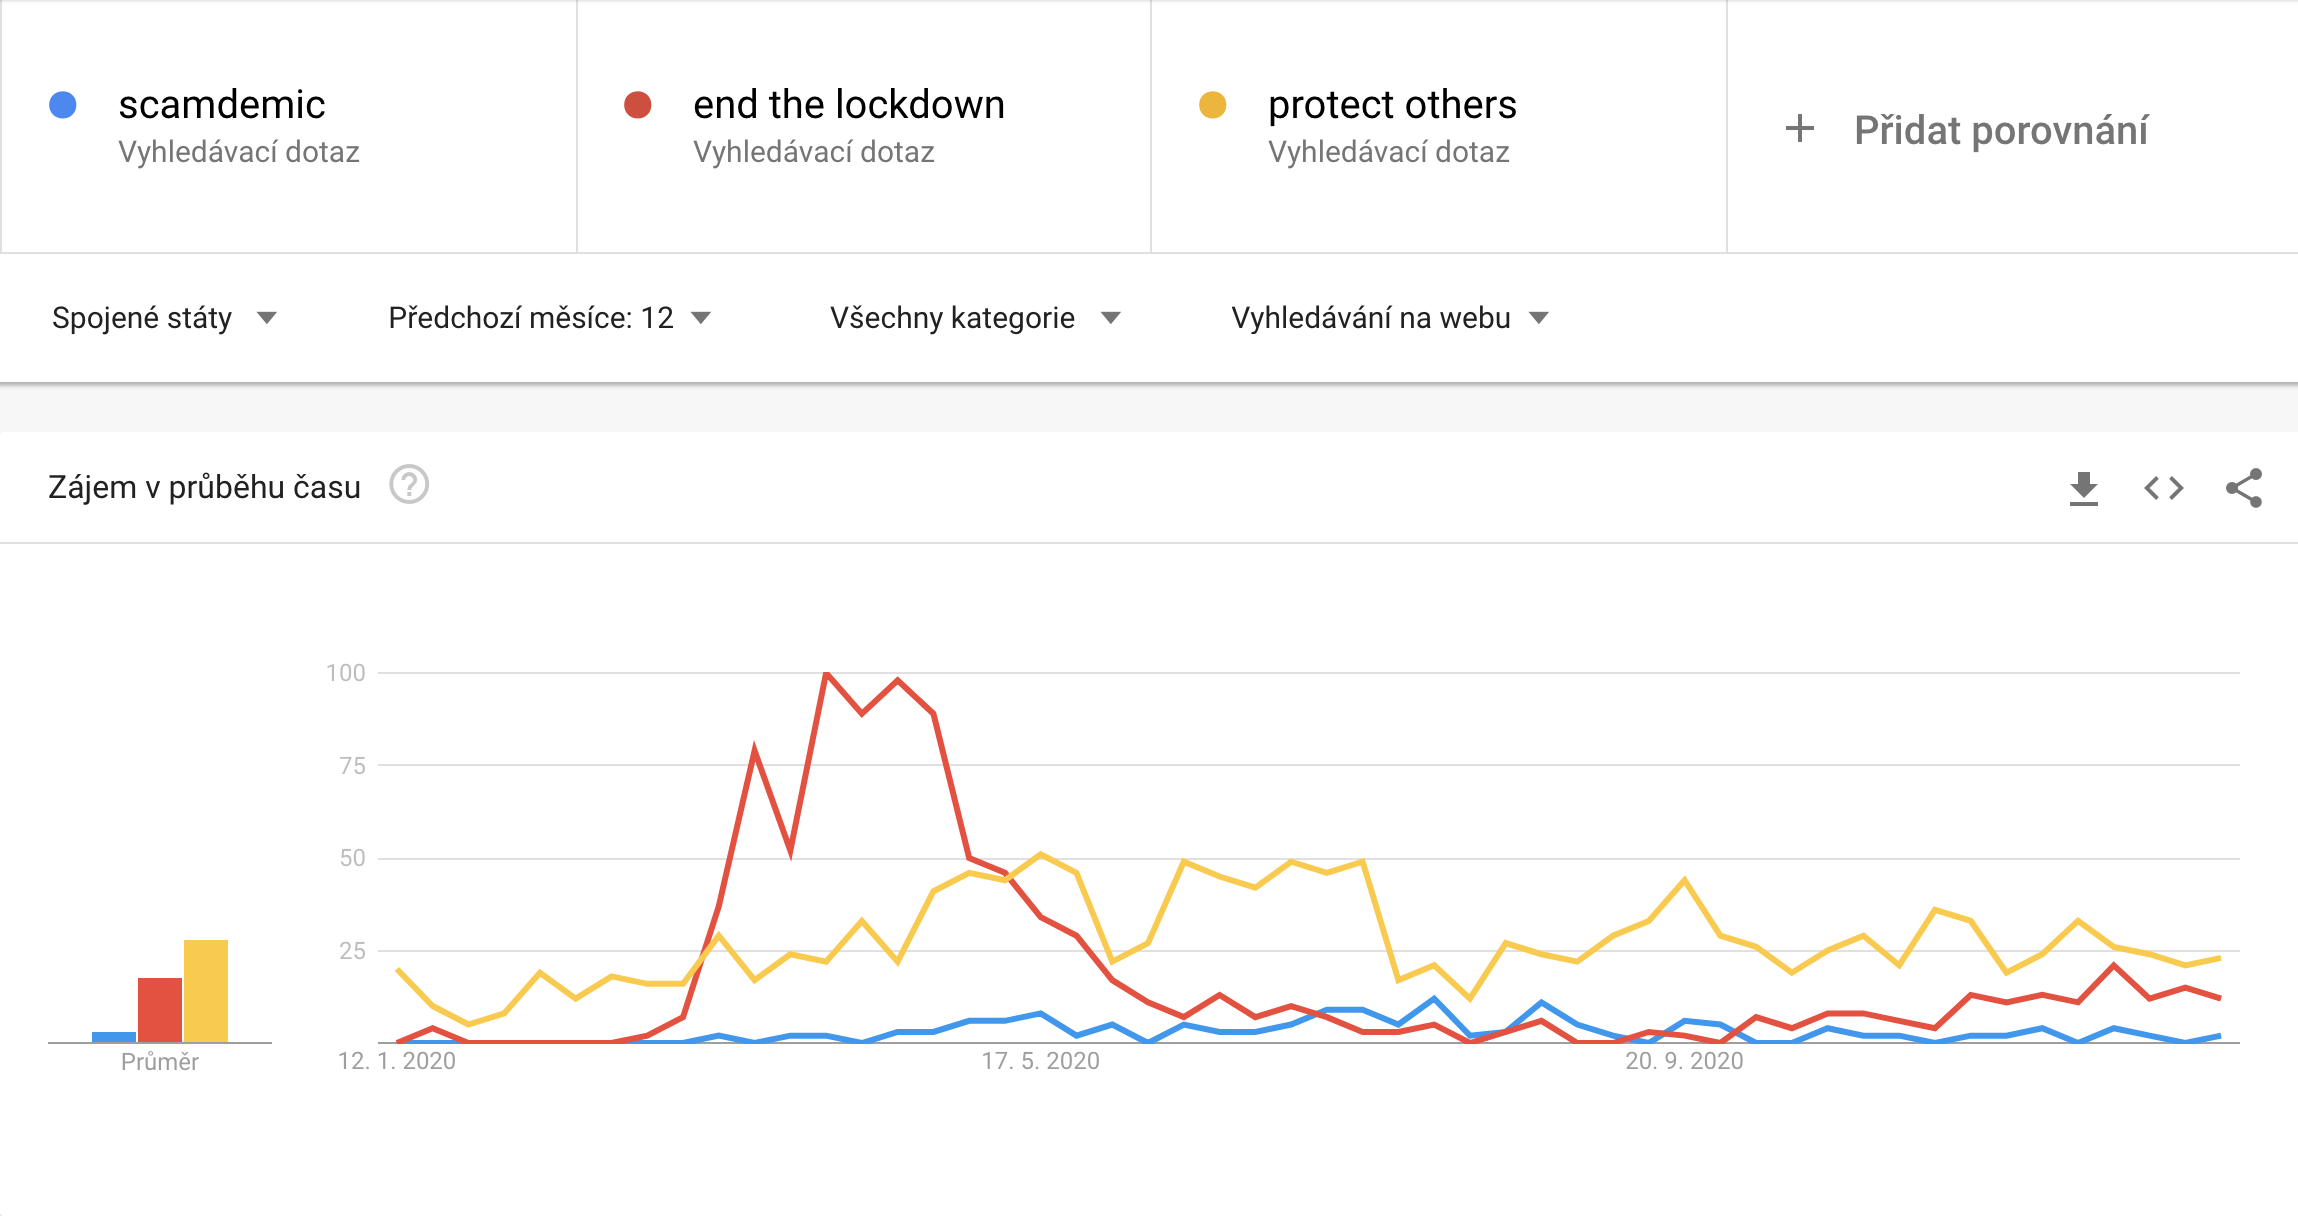
\includegraphics[width=14cm]{google_trends_analysis.png}
  \caption{Obrázek}
  \label{fig:tux}
\end{figure}

\section{Jak proti dezinformacím bojovat?}

\section{Závěr}